%
% strahlung.tex
%
% (c) 2018 Prof Dr Andreas Müller, Hochschule Rapperswil
%
\section{Strahlung\label{section:strahlung}}
\rhead{Strahlung}
Die von der Erde empfange Strahlung sowie die Albedo wurden bereits in
Abschnitt~\ref{skript:grundlagen:strahlung} untersucht.
Für die später in diesem Kapitel zu untersuchenden Modelle ist aber
erforderlich, die örtliche Verteilung der Strahlung auf der Erdoberfläche
genauer zu verstehen.
In diesem Abschnitt wird daher zuerst die Strahlungsleistung auf einer
Halbkugel und später auf einer Zone um einen Breitenkreis berechnet.
%
% halbkugel.tex -- Einstrahlung auf eine Halbkugel
%
% (c) 2018 Prof Dr Andreas Müller, Hochschule Rapperswil
%
\subsection{Einstrahlung auf einer Halbkugel\label{subsection:halbkugel}}
\begin{figure}
\centering
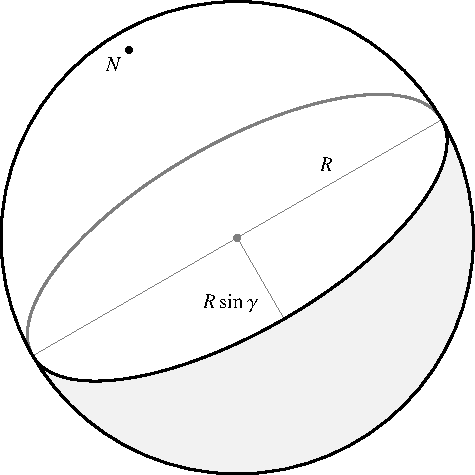
\includegraphics{chapters/5/halb.pdf}
\caption{Aufteilung der sonnenbeschienenen Seite der Erde durch den
Äquator.
\label{skript:halbkugel:teilung}}
\end{figure}%
Die einfachste Erweiterung des Modells von Budyko teilt die
Erde in zwei Halbkugeln auf, die Energie nur langsam austauschen
können.
Für die Energiebilanz brauchen wir daher die Strahlungsleistung
auf einer Halbkugel in Abhängigkeit von der Neigung $\gamma$ der
Erdachse.

Die gesamte auf auf die Erde eingestrahlte Leistung ist $\pi R^2S_0$.
Diese Leistung muss nun in Abhängigkeit von der Neigung $\gamma$
auf die beiden Halbkugeln verteilt werden.
Von der Erde aus gesehen teilt der Äquator die bestrahlte Erde wie
in Abbildung~\ref{skript:halbkugel:teilung} dargestellt.
Der Unterschied zwischen den beiden Halbkugeln ist der Flächeninhalt
der Ellipse, also
\[
F=\pi R^2\sin\gamma.
\]
Die Strahlungsleistung auf den beiden Halbkugeln in
Abbildung~\eqref{skript:halbkugel:teilung} ist daher
\begin{align}
E_N
&= 
\frac12(\pi R^2 S_0 +\pi R^2S_0\sin\gamma)
=
\pi R^2S_0 \frac{1+\sin\gamma}2 = Q\frac{1+\sin\gamma}2
&&\text{Nordhalbkugel,}
\\
E_S
&= 
\frac12(\pi R^2 S_0 -\pi R^2\sin\gamma)
=
\pi R^2S_0 \frac{1-\sin\gamma}2 = Q\frac{1-\sin\gamma}2
&&\text{Südhalbkugel.}
\end{align}
In Kapitel~\ref{chapter:neigung} wird diese Lösung verwendet, um zu
modellieren, wie die Veränderung der Neigung der Erdachse zu Eiszeiten
führen kann.





%
% einstrahlung.tex
%
% (c) 2018 Prof Dr Andreas Müller,Hochschule Rapperswil
%
\subsection{Einstrahlung auf einen Breitenkreis}
Wir berechnen die Einstrahlung auf einem gegebenen Breitengrad
$\vartheta$ in Abhängigkeit von der Neigung $\gamma$
der Erdachse.
Die einfallende Strahlungsleistung ist proportional zum Skalarprodukt
der Richtung der Einstrahlung mit der Normalen in einem Punkte
auf dem Breitenkreis zur Breite $\vartheta$.
Die Normale ist
\[
\vec n(\vartheta,\varphi)
=
\begin{pmatrix}
\sin\vartheta\cos\varphi\\
\sin\vartheta\sin\varphi\\
\cos\vartheta
\end{pmatrix}.
\]
Die Richtung der Einstrahlungsrichtung ist
\[
\vec e(\gamma)
=
\begin{pmatrix}
\cos\gamma\\
0\\
\sin\gamma
\end{pmatrix}.
\]
Das Skalarprodukt ist
\begin{equation}
\vec n(\vartheta,\varphi)\cdot\vec e(\gamma)
=
\sin\vartheta\cos\varphi\cos\gamma
+
\cos\vartheta\sin\gamma.
\label{skript:einstrahlung:skalarprodukt}
\end{equation}
Für die folgende Diskussion nehmen wir an, dass $\gamma >= 0$,
dass also der Nordpol permanent bestrahlt ist und der Südpol keine
Strahlung erhält.

Im Folgenden wollen wir die Energie berechnen, die in eine Zone
eingestrahlt wird.

\subsubsection{Sonnenauf- und -untergang}
Die Einstrahlung erfolgt natürlich nur zwischen Sonnenauf- und
-untergang.
Wir bezeichen die geographische Länge, bei der der Sonnenauf- oder
-untergang erfolgt, mit $\pm\varphi_0$.
Diese sind gekennzeichnet dadurch, dass $\vec n(\vartheta,\varphi_0)$ und
$\vec e(\gamma)$ senkrecht aufeinander stehen oder
\begin{equation*}
\begin{aligned}
&&
\vec n(\vartheta,\varphi_0)&\perp \vec e(\gamma)
\\
&\Rightarrow&
\vec n(\vartheta,\varphi_0)\cdot \vec e(\gamma)&=0
\\
&\Rightarrow&
\sin\vartheta\cos\varphi_0\cos\gamma
&=
-
\cos\vartheta\sin\gamma
\\
&\Rightarrow&
\cos\varphi_0
&=
-\frac{\tan\gamma}{\tan\vartheta}.
\end{aligned}
\end{equation*}
Wenn $\vartheta < \gamma$ (Punkt in der Nähe des Nordpols) oder
$\vartheta > \pi - \gamma$ (Punkt in der Nähe des Südpols),
dann hat die Gleichung keine Lösung,
die Sonne geht nie auf (Polarnacht) oder unter (Polartag).

\subsubsection{Mittlere Strahlungsleistung auf Breite $\vartheta$}
Um die Strahlungsleistung auf einer beliebigen geographischen
Breite zu berechnen, gehen wir in zwei Schritten vor.
Das Skalarprodukt~\eqref{skript:einstrahlung:skalarprodukt} 
gibt die Strahlungsleistung $\varepsilon(\vartheta,\varphi,\gamma)$
in einem Punkt auf der geographischen
Breite $\vartheta$ in Abhängigkeit von $\varphi$.
Im ersten Schritt mitteln wir dies über eine Umdrehung, dazu
ist das Skalarprodukt~\eqref{skript:einstrahlung:skalarprodukt} über eine
Umdrehung zu mitteln.
So erhalten wir die mittlere Strahlungsleistung $\varepsilon(\vartheta,\gamma)$
in einem Punkte auf geographischer Breite $\vartheta$.
Im zweiten Schritt müssen wir die die mittlere Strahlungsleistung mit
der Länge des Breitenkreises multiplizieren, um die Strahlungsleistung
auf dem Breitenkreis zur Breite $\vartheta$ zu erhalten.

\subsubsection{Polnähe}
In der Nähe des Südpols, also wenn $\vartheta > \pi - \gamma$,
ist die Einstrahlung $=0$.
In der Nähe des Nordpols, also wenn $\vartheta < \gamma$, ist die
Einstrahlungsdichte
\[
\varepsilon_{\text{in}}
=
\int_0^{2\pi}
\sin\vartheta\cos\varphi\cos\gamma
+
\cos\vartheta\sin\gamma
\,d\varphi
=
2\pi\cos\vartheta\sin\gamma.
\]
Für den Spezialfall $\vartheta=0$ fällt der erste Term weg und es
bleibt 
\begin{align*}
\varepsilon_{\text{in}}(0,\gamma)
&=
2\pi\sin\gamma.
\end{align*}

\subsubsection{Äquator}
Am Äquator ist $\vartheta=\frac{\pi}2$ und $\varphi_0=\frac{\pi}2$.
Man bekommt
\begin{align*}
\varepsilon_{\text{in}}\biggl(\frac{\pi}2,\gamma\biggr)
&=
\int_{-\varphi_0}^{\varphi_0}
\cos\varphi\cos\gamma\,d\varphi
=
\cos\gamma
\int_{-\frac{\pi}2}^{\frac{\pi}2}
\cos\varphi
\,d\varphi
=
2\cos\gamma
\end{align*}
für die Einstrahlung am Äquator.

\subsubsection{Der allgemeine Fall mit Sonnenauf- und -untergang}
\begin{figure}
\centering
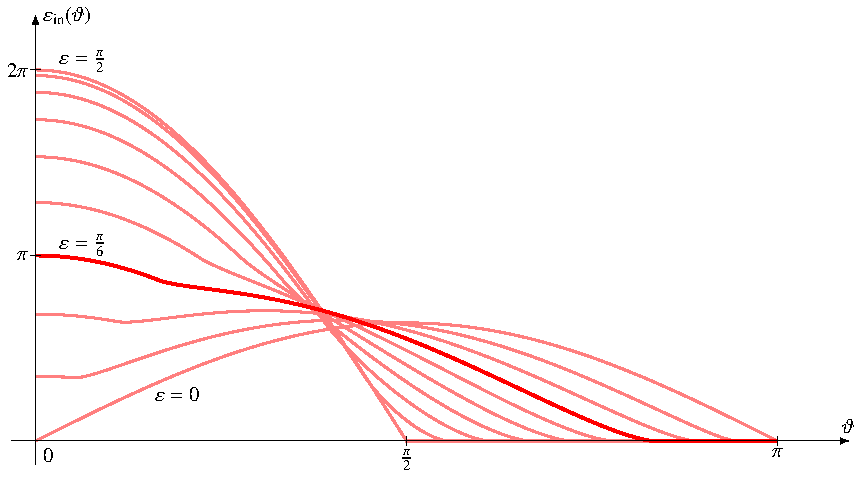
\includegraphics[width=\hsize]{chapters/5/ein.pdf}
\caption{Über eine Rotation gemittelte Einstrahlungsdichte
in Abhängigkeit von der geographischen Breite
gemäss Formel~\eqref{skript:einstrahlung:plottable} für verschiedene
Neigungen $\gamma$ der Achse. 
Dargestellt sind $\gamma$-Werte zwischen 0 und $90^\circ$ 
in $10^\circ$-Schritten. 
Die Neigung $\gamma=30^\circ=\frac{\pi}{6}$ ist hervorgehoben.
\label{skript:einstrahlung:ein}}
\end{figure}%
Der allgemeine Fall mit Sonnenauf- und -untergang
ist $\gamma < \vartheta < \pi-\gamma$.
Für die Einstrahlung finden wir dann
\begin{align}
\varepsilon_{\text{in}}(\vartheta,\gamma)
&=
\int_{-\varphi_0}^{\varphi_0}
\sin\vartheta\cos\varphi\cos\gamma
+
\cos\vartheta\sin\gamma\,d\varphi
\notag
\\
&=
\sin\vartheta\cos\gamma\biggl[\sin\varphi\biggr]_{-\varphi_0}^{\varphi_0}
+
2\varphi_0 \cos\vartheta\sin\gamma
\notag
\\
&=
2\sin\vartheta\cos\gamma\sin\varphi_0
+
2\varphi_0 \cos\vartheta\sin\gamma
\notag
\\
&=
2\sin\vartheta\cos\gamma
\sin
\arccos\biggl(-\frac{\tan\gamma}{\tan\vartheta}\biggr)
+
2\cos\vartheta\sin\gamma
\arccos\biggl(-\frac{\tan\gamma}{\tan\vartheta}\biggr).
\notag
\\
\intertext{Im ersten Term können wir $\sin\arccos x  = \sqrt{1-x^2}$
verwenden.
Den zweiten Term könnten wir so stehen lassen, aber für die graphische
Darstellung brauchen wir eine Darstellung das Arkuskosinus durch den
Arkustangens, da TikZ nur den Arkustangens anbietet.
Wir verwenden die Formel $\arccos x = 2\arctan\sqrt{(1-x)/(1+x)}$ und
erhalten}
&=
2\sin\vartheta\cos\gamma
\sqrt{1-\frac{\tan^2\gamma}{\tan^2\vartheta}}
+
4\cos\vartheta\sin\gamma
\arctan\sqrt{\frac{1+\frac{\tan\gamma}{\tan\vartheta}}{1-\frac{\tan\gamma}{\tan\vartheta}}}
\notag
\\
&=
\pm2\cos\vartheta\cos\gamma
\sqrt{\tan^2\vartheta-\tan^2\gamma}
+
4\cos\vartheta\sin\gamma
\arctan\sqrt{\frac{\tan\vartheta+\tan\gamma}{\tan\vartheta-\tan\gamma}}
\notag
\\
&=
2
\cos\vartheta
\biggl(
\cos\gamma
\sqrt{\frac{\tan^2\vartheta}{\tan^2\gamma}-1}
+
2
\sin\gamma
\arctan\sqrt{
\frac{\tan\vartheta+\tan\gamma}{\tan\vartheta-\tan\gamma}
}
\biggr).
\label{skript:einstrahlung:plottable}
\end{align}
Formel~\eqref{skript:einstrahlung:plottable} ist in
Abbildung~\ref{skript:einstrahlung:ein} dargestellt.

\subsubsection{Strahlungsleistung auf dem Breitenkreis $\vartheta$}
\begin{figure}
\centering
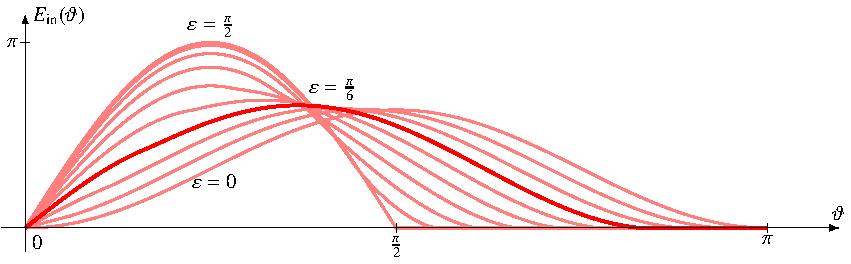
\includegraphics[width=\hsize]{chapters/5/ein1.pdf}
\caption{Strahlungsleistung auf geographischer Breite $\vartheta$,
gegeben durch Formel~\eqref{skript:einstrahlung:breite}.
\label{skript:einstrahlung:ein1}}
\end{figure}%
Die gesamte Strahlungsleistung auf dem Breitenkreis $\vartheta$
ist
\begin{equation}
E_{\text{in}}(\vartheta)
=
\varepsilon(\vartheta,\gamma)
\cdot
\sin\vartheta
\label{skript:einstrahlung:breite}
\end{equation}
Die resultierende Funktion ist in Abbildung~\ref{skript:einstrahlung:ein1}
dargestellt.

\subsection{Einstrahlung über ein Jahr}
\begin{figure}
\centering
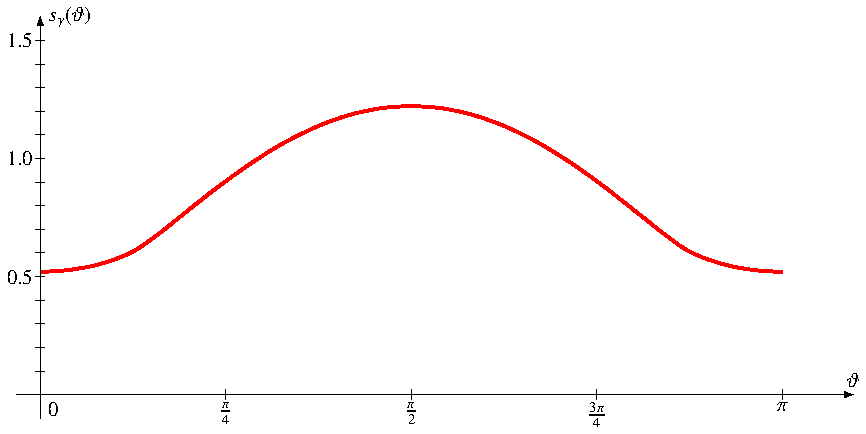
\includegraphics[width=\hsize]{chapters/5/total.pdf}
\caption{Einstrahlung über ein Jahr in Abhängigkeit von der geographischen
Breite.
\label{skript:einstrahlung:total}}
\end{figure}
Die in \eqref{skript:einstrahlung:breite} gefunden Einstrahlung auf einem
Breitengrad $\vartheta$ geht von einer konstanten Neigung der Erdachse aus.
Die Bewegung der Erde um die Sonne bedeutet aber, dass die Neigung der
der Erdachse scheinbar variert,
es gilt nämlich
\[
\tan \gamma(t) = \tan\gamma_\text{max}\cdot \sin t.
\]
Für ein Klimamodell wesentlich ist daher der Mittelwert
\[
s_{\gamma_\text{max}}(\vartheta)
=
\frac1{2\pi}
\int_0^{2\pi} \varepsilon(\vartheta,\gamma(t))\,dt
\]
von \eqref{skript:einstrahlung:breite} über ein Jahr.
Abbildung~\ref{skript:einstrahlung:total} zeigt das Resultat der 
numerischen Integration.









